\documentclass[12pt,aspectratio=1610]{beamer}
\RequirePackage{
    amsmath,
    amssymb,
    calc,
    cancel,
    booktabs,
    color,
    siunitx,
    tikz,
    wrapfig,
    array,
    leftidx,
    float,
    etoolbox,
    fancyhdr,
    longtable,
    hyperref,
    ltcaption,
    ulem,
    wasysym,
    accents,
    listings,
    tabularx,
}

\hypersetup{
    hidelinks,
    breaklinks              = true,
}

\usepackage[final]{pdfpages}
\usepackage[many]{tcolorbox}

\RenewDocumentCommand{\vec}{m}{\mathbf{#1}}

\makeatletter
    \def\new@mathgroup{\alloc@8\mathgroup\mathchardef\@cclvi}
    \patchcmd{\document@select@group}{\sixt@@n}{\@cclvi}{}{}
    \patchcmd{\select@group}{\sixt@@n}{\@cclvi}{}{}
\makeatother

\RequirePackage{mathspec}                                   % includes fontspec
\RequirePackage{polyglossia}                                % multi-language support
\RequirePackage{xunicode}
\setdefaultlanguage{slovak}

% Setup fonts -- see fontspec/mathspec documentation.
\defaultfontfeatures{
    Mapping         = tex-text,
    Scale           = MatchLowercase,
    Ligatures       = TeX
}


\NewDocumentCommand{\labelmath}{m +m}{%
    \begin{equation}%
        #2%
        \label{#1}%
    \end{equation}%
}

\NewDocumentCommand{\labelalign}{m +m}{%
    \begin{align}%
        #2%
        \label{#1}%
    \end{align}%
}

\linespread{1.0}
\setlength{\parindent}{0cm}
\setlength{\parskip}{6pt}
\setlength{\abovedisplayskip}{0mm}
\setlength{\belowdisplayskip}{0mm}
\setlength{\abovedisplayshortskip}{0mm}
\setlength{\belowdisplayshortskip}{0mm}
\setlength{\itemindent}{0pt}
\setlength{\textfloatsep}{0mm}
\setlength{\tabcolsep}{3mm}
\setlength{\LTcapwidth}{0.8\textwidth}
\renewcommand{\arraystretch}{1.2}

\setcounter{secnumdepth}{2}

/home/kvik/dgs/core/tex/math.tex
\DeclareSIUnit\au{AU}
\DeclareSIUnit\pixel{px}
\DeclareSIUnit\lightyear{ly}
\DeclareSIUnit\parsec{pc}
\DeclareSIUnit\earthmass{M_{\earth}}
\DeclareSIUnit\speedoflight{c}
\DeclareSIUnit\foe{foe}
\DeclareSIUnit\year{yr}
\DeclareSIUnit\eur{€}
\DeclareSIUnit\solarmass{M_{\astrosun}}
\DeclareSIUnit\solarluminosity{L_{\astrosun}}
\DeclareSIUnit{\byte}{B}




\linespread{1.0}
\setlength{\parindent}{0cm}
\setlength{\parskip}{6pt}
\setlength{\abovedisplayskip}{0mm}
\setlength{\belowdisplayskip}{0mm}
\setlength{\abovedisplayshortskip}{0mm}
\setlength{\belowdisplayshortskip}{0mm}
\setlength{\itemindent}{0pt}
\setlength{\textfloatsep}{0mm}
\setlength{\tabcolsep}{3mm}
\renewcommand{\arraystretch}{1.2}

\setcounter{secnumdepth}{0}

\NewDocumentCommand{\fspicture}{m O{W} O{black}}{
    {
        \setbeamertemplate{navigation symbols}{}
        \setbeamercolor{background canvas}{bg = #3}
        \begin{frame}[plain]
            \begin{tikzpicture}[remember picture, overlay]
                \node[at=(current page.center)] {
                    \ifstrequal{H}{#2}{                                  
                        \includegraphics[height=\paperheight]{#1}%
                    }{%
                        \includegraphics[width=\paperwidth]{#1}%
                    }
                };
            \end{tikzpicture}
        \end{frame}
    }
}

\NewDocumentCommand{\frejm}{m +m}{
    \begin{frame}
        \frametitle{#1}
        #2
    \end{frame}
}

\NewDocumentCommand{\fragfrejm}{m +m}{
    \begin{frame}[fragile]
        \frametitle{#1}
        #2
    \end{frame}
}

\defbeamertemplate{description item}{align center}{\hfill\insertdescriptionitem\hfill}
\definecolor{desc}{rgb}{0.66, 0, 0}
\definecolor{citem}{rgb}{0.72, 0, 0}
\definecolor{csitem}{rgb}{0.90, 0, 0}
\definecolor{cssitem}{rgb}{1, 0.1, 0.1}
\definecolor{qprimarybg}{rgb}{0.95, 0.95, 0.95}
\definecolor{check}{rgb}{0, 0.8, 0}
\definecolor{coded}{rgb}{0.9, 0.9, 0.9}
\definecolor{todo}{rgb}{1.0, 0.3, 0.3}
\definecolor{model}{rgb}{0.75, 0, 0}

\setbeamertemplate{navigation symbols}{}
\newfontfamily{\semibold}{Segoe UI Semibold}
\RenewDocumentCommand{\emph}{m}{{\semibold#1}}
\NewDocumentCommand{\code}{m}{\textcolor{desc}{\texttt{#1}}}
\NewDocumentCommand{\model}{m}{\colorbox{coded}{\textcolor{model}{\texttt{#1}}}}
\NewDocumentCommand{\todo}{m}{\colorbox{todo}{#1}}

\mode<presentation> {
    \usetheme{Szeged}
    \usecolortheme{beaver}
    
    \usefonttheme{professionalfonts}
    \setallmainfonts{Minion Pro}
    \setmathrm{Minion Pro}
    
    \setsansfont{Segoe UI}
    \setmonofont{Consolas}
    \setbeamercolor*{enumerate item}{fg = citem}
    \setbeamercolor*{enumerate subitem}{fg = csitem}
    \setbeamercolor*{enumerate subsubitem}{fg = cssitem}
    \setbeamercolor*{description item}{fg = desc}
    \setbeamercolor*{itemize item}{fg = citem}
    \setbeamercolor*{itemize subitem}{fg = csitem}
    \setbeamercolor*{itemize subsubitem}{fg = cssitem}
    \setbeamercolor*{palette primary}{fg = red, bg = qprimarybg}
}

\newcommand<>\highlightbox[2]{%
    \alt#3{\makebox[\dimexpr\width-2\fboxsep]{\colorbox{#1}{#2}}}{#2}%
}

\AtBeginSection[]{
    \subsection{\insertsection}
    \begin{frame}
        \vfill
        \centering
        \begin{beamercolorbox}[sep = 18pt, center, shadow = true, rounded = true]{title}
            \usebeamerfont{title}\insertsectionhead%
            \vfill
        \end{beamercolorbox}
        \vfill
    \end{frame}
}

\makeatletter
% Render percent sign with nice font, not ugly Computer modern
    \mathcode`\%="7025

% Fixes mathspec bug -- URL numbers are rendered with wrong font
    \ernewcommand\eu@MathPunctuation@symfont{Latin:m:n}
    \DeclareMathSymbol{,}{\mathpunct}{\eu@MathPunctuation@symfont}{`,}
    \DeclareMathSymbol{?}{\mathpunct}{\eu@MathPunctuation@symfont}{`?}
    \DeclareMathSymbol{.}{\mathord}{\eu@MathPunctuation@symfont}{`.}
    \DeclareMathSymbol{<}{\mathrel}{\eu@MathPunctuation@symfont}{`<}
    \DeclareMathSymbol{>}{\mathrel}{\eu@MathPunctuation@symfont}{`>}
    \DeclareMathSymbol{/}{\mathord}{\eu@MathPunctuation@symfont}{`/}
    \DeclareMathSymbol{;}{\mathpunct}{\eu@MathPunctuation@symfont}{`;}
    \DeclareMathSymbol{(}{\mathopen}{\eu@DigitsArabic@symfont}{`(}
    \DeclareMathSymbol{)}{\mathclose}{\eu@DigitsArabic@symfont}{`)}
    \XeTeXDeclareMathSymbol{^^^^2026}{\mathinner}{\eu@MathPunctuation@symfont}{"2026}[\mathellipsis]
    \DeclareMathSymbol{0}{\mathalpha}{\eu@DigitsArabic@symfont}{`0}
    \DeclareMathSymbol{1}{\mathalpha}{\eu@DigitsArabic@symfont}{`1}
    \DeclareMathSymbol{2}{\mathalpha}{\eu@DigitsArabic@symfont}{`2}
    \DeclareMathSymbol{3}{\mathalpha}{\eu@DigitsArabic@symfont}{`3}
    \DeclareMathSymbol{4}{\mathalpha}{\eu@DigitsArabic@symfont}{`4}
    \DeclareMathSymbol{5}{\mathalpha}{\eu@DigitsArabic@symfont}{`5}
    \DeclareMathSymbol{6}{\mathalpha}{\eu@DigitsArabic@symfont}{`6}
    \DeclareMathSymbol{7}{\mathalpha}{\eu@DigitsArabic@symfont}{`7}
    \DeclareMathSymbol{8}{\mathalpha}{\eu@DigitsArabic@symfont}{`8}
    \DeclareMathSymbol{9}{\mathalpha}{\eu@DigitsArabic@symfont}{`9}
\makeatother


\title{Reflectance spectroscopy with GTC}
\subtitle{}
\author{\small \emph{Martin Baláž}}
\institute{DAA coffee}
\date{2020--07--01}

\begin{document}
    {
        \usebackgroundtemplate{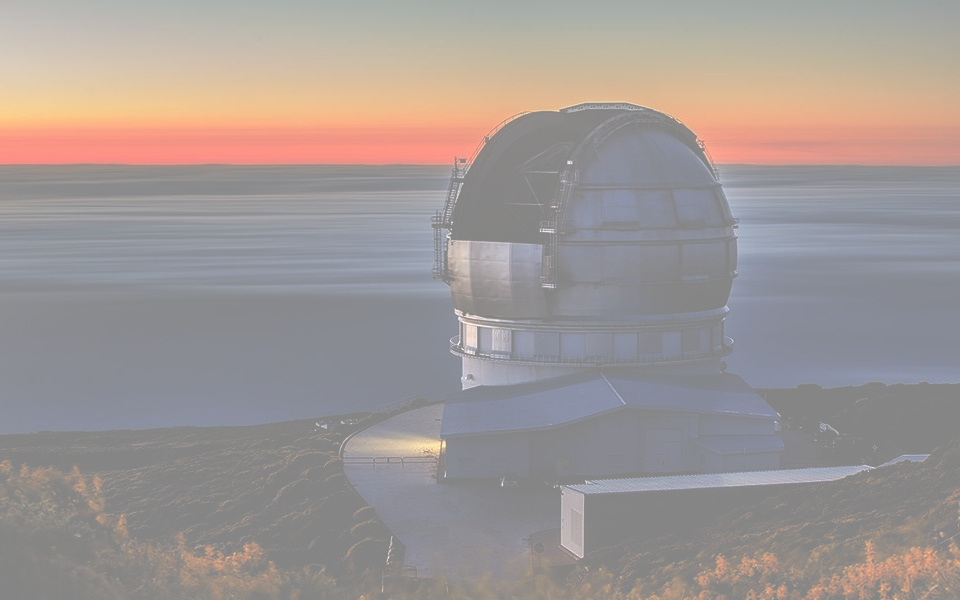
\includegraphics[width=\paperwidth]{pictures/gtc.jpg}}
        \begin{frame}
            \titlepage
        \end{frame}
    }

    \section{OSIRIS}
        \frejm{OSIRIS}{
            čo to je?
        }

        \frejm{\texttt{IRAF} and \texttt{Starlink}}{
            \begin{columns}
                \begin{column}{0.5\textwidth}
                    \begin{itemize}
                        \item IRAF
                            \begin{itemize}
                                \item US NOAO, since 1985
                                \item horrible installation
                                \item last release 2012
                                \item usage in new projects discouraged
                            \end{itemize}
                        \pause
                        \item Starlink
                            \begin{itemize}
                                \item the same but very British
                                \item \SI{1}{\giga\byte} of... something
                                \item slightly newer
                            \end{itemize}
                    \end{itemize}
                \end{column}
                \pause
                \begin{column}{0.4\textwidth}
                    
\includegraphics[width=\linewidth]{pictures/dinosaur-computer.jpg}
                \end{column}
            \end{columns}
        }

        \frejm{\texttt{THELI} and \texttt{ccdproc}}{
            Let us use something newer...
            \begin{itemize}
                \item Theli
                    \begin{itemize}
                        \item new German software
                        \item highly recommended for general purpose reduction
                    \end{itemize}
                \pause
                \item \texttt{ccdproc}
                    \begin{itemize}
                        \item not a \emph{program}, but a \emph{Python library}
                        \item well documented
                        \item great for pipelline integration
                    \end{itemize}
            \end{itemize}
        }

        \frejm{Osiris reduction pipeline}{
            Basic operations but fine-tuned for this purpose
            \begin{itemize}
                \item preprocessing
                    \begin{itemize}
                        \item master bias
                        \item master flat
                        \item trimming
                    \end{itemize}
                \pause
                \item extraction of the spectrum
                    \begin{itemize}
                        \item identification
                        \item background
                        \item cosmic rays
                    \end{itemize}
                \item normalization
                    \begin{itemize}
                        \item spectral flat field
                        \item divide by solar analogue spectrum
                    \end{itemize}
            \end{itemize}
        }

    \section{Geofit}
        \frejm{Geofit}{
            \begin{itemize}
                \item program by Ted Roush
                \item FORTRAN77
                \item written in January 1992
                \pause
                \item uses \emph{Hapke model} to compute synthetic reflectance spectra
                \item comparison to observational spectra
                \pause
                \item virtually no comments
                \item untouched since 2012
            \end{itemize}
        }

        \frejm{Objective}{
            \begin{columns}
                \begin{column}{0.7\textwidth}
                    \begin{itemize}
                        \item make at least some sense of it
                        \item rewrite in \texttt{Python}
                        \item optimize
                        \pause
                        \item job halfway between \emph{programming} and \emph{archaeology}
                    \end{itemize}
                \end{column}
                \begin{column}{0.28\textwidth}
                    
\includegraphics[width=\linewidth]{pictures/frankenstein.jpg}
                \end{column}
            \end{columns}
        }

        \frejm{Operation}{
            \begin{columns}
                \begin{column}{0.7\textwidth}
                    \begin{itemize}
                        \item \emph{ab initio} model of BRDF $f_r(\omega_i, \omega_r)$
                        \item material mixtures, interpolation of spectral values
                        \begin{itemize}
                            \item intimate
                            \item spatial
                        \end{itemize}
                        \pause
                        \item Nelder-Mead minimization of the objective function ($\chi^2$)
                        \item database of materials
                    \end{itemize}
                \end{column}
                \begin{column}{0.28\textwidth}
                    
\includegraphics[width=\linewidth]{pictures/brdf.png}
                \end{column}
            \end{columns}
        }


    \section{Summary}
        \frejm{References}{
            \begin{itemize}
                \item GTC image: Daniel López, \texttt{elcielodecanarias.com}
            \end{itemize}
        }
\end{document}
